
\documentclass[twocolumn]{article}
\usepackage{mathpazo}
\usepackage{microtype}
\usepackage{times}

 %%%%%%%%%%%%%%%%%%%%%%%%%%%%%%%%%%%%%%%%%%%%%%%%%%%%%%%%%%%%%%%%%%%%%%%%%%%%%
 %                              My Commands
\newcommand{\bi}{\begin{itemize}}
\newcommand{\ei}{\end{itemize}}
\newcommand{\be}{\begin{enumerate}}
\newcommand{\ee}{\end{enumerate}}
\newcommand{\ii}{\item}
\newtheorem{Def}{Definition}
\newtheorem{Lem}{Lemma}
\usepackage{algorithm}
\usepackage{algorithmicx}
\usepackage{algpseudocode}

\usepackage{graphicx}
\graphicspath{%
        {converted_graphics/}
        {./images/}
}
    
\setlength\textwidth{7in} 
\setlength\textheight{9.5in} 
\setlength\oddsidemargin{-0.25in} 
\setlength\topmargin{-0.25in} 
\setlength\headheight{0in} 
\setlength\headsep{0in} 
\setlength\columnsep{18pt}
\sloppy 
 
\begin{document}

\title{
\vspace{-0.5in}\rule{\textwidth}{2pt}
\begin{tabular}{ll}\begin{minipage}{4.75in}\vspace{6px}
\noindent\large Autonomous Control Middleware Research Section\\
\vspace{-12px}\\
\noindent\LARGE ETRI\qquad \large Technical Report 13VC1310-TR-11
\end{minipage}&\begin{minipage}{2in}\vspace{6px}\small
218 Gajeong-ro, Yuseong-gu\\
Daejeon, 305-700, South Korea\\
http:/$\!$/www.etri.re.kr/\quad 
\end{minipage}\end{tabular}
\rule{\textwidth}{2pt}\vspace{0.25in}
\LARGE \bf
Middleware Architecture
}

%\date{Autonomous Control Middleware Research Section, ETRI}
\date{}

\author{
{\bf Sung-Soo Kim}\\
\it{sungsoo@etri.re.kr}
}

\maketitle

\begin{abstract}

Smart devices with wireless communication interfaces  such as smart TV, smart tablets or smart phones  are becoming more powerful and commonplace. Consequently, demand has increased for applications and services that support communication and collaboration among mobile users. This new distributed computing environment poses new challenges, such as host mobility, limited device resources, and intermittent connectivity. However, it also opens up a range of different and unexplored forms of collaboration among mobile users, in which, for example, information about user locality and proximity could play a distinguished role in determining an interaction's form and participants.

\end{abstract}

\section{Introduction}

We argue that collaboration in a static network differs significantly from collaboration in a mobile network. While for collaboration based on static networks, one implicitly assumes that all user devices have stable connectivity, this isn't the case in a mobile environment. Because mobile networks suffer from weak and intermittent connectivity, a user might become temporarily unavailable even though he or she is still engaged in the collaboration session. Hence, in a mobile setting, the requirements for synchronous views and mutual perception for the collaborating peers (collaboration awareness) needs to be redefined.

Another difference is related to user mobility. When users are mobile, the collaborating group tends to be more dynamic and arises spontaneously, motivated by a shared common interest or situation. Moreover, the way a mobile user interacts with other community or group members tends to be more variable, asynchronous, and dependent on the user's current context, activity, or interest.
Finally, collaboration between mobile users usually isn't driven by a global and predefined goal or task, such as cooperative work on a digital or physical artifact. Instead, it's driven by spontaneous and occasional initiatives for mutual sharing of information, contribution to the development or improvement of public knowledge, and so on. This makes participation in a collaboration more spontaneous and irregular, and usually motivated by implicitly (or explicitly) assessed gain of reputation owing to the contribution of higher-quality, more precise, or more relevant information.

All the aforementioned characteristics suggest that environments for developing mobile collaboration applications and services should incorporate new mechanisms that would facilitate collecting, aggregating, and accessing (at the application level) different kinds of information about the individual and collective contexts of collaborating users. This information can become directly available to the collaborating peers (for example, for enhancing the group's collaboration awareness) or can be used for adapting the application's behavior (for example, its available functions or user interfaces) to the current situation.
MoCA (mobile collaboration architecture) is a middleware architecture for developing context- processing services and context-sensitive applications for mobile collaboration. Our work on this architecture is part of a wider project that aims to experiment with new forms of mobile collaboration and implement a flexible and extensible service-based environment for developing collaborative applications for infrastructured mobile networks.

The MoCA infrastructure consists of client and server APIs, basic services supporting collaborative applications, and a framework for implementing application proxies (the ProxyFramework). Each application has three types of elements: servers, proxies, and clients. The first two execute on nodes of the static network, while clients run on mobile devices. The proxy intermediates all communication between the application servers and the clients. Applications with requirements to scale to numerous clients might have several proxies executing on different networks. An application's proxy could be in charge of several tasks, such as adapting the transferred data  for example, applying data compression, protocol conversion, encryption, user authentication, context processing, service discovery, handover management, and others. Most of these tasks require significant processing effort, so the proxy is also a way to distribute the application-specific processing among the server and its proxies.

A collaborative application's server and client should be implemented using the MoCA APIs because they hide from the application developer most details concerning the interactions with the services that the architecture provides (which we discuss in the next section). We designed the APIs and the basic services to be generic and flexible, so they'd be useful for different types of collaborative applications  for example, those based on synchronous or asynchronous, message- or sharing-oriented communication.

The ProxyFramework--a white-box framework--can be used to create application proxies according to the collaborative application's specific needs. It facilitates access to MoCA's basic services and the programming of application-specific adaptations triggered by events related to context changes.
In MoCA, most of these tasks require significant processing effort, so the proxy is also a way to distribute the application-specific processing among the server and its proxies.
Additionally, the architecture offers the following components and core services, which support the development of context-aware collaborative applications.

The monitor is a daemon executing on each mobile device. It collects data concerning the device and network's state and sends this data to the context information service (CIS) executing on one or more nodes of the wired network. The collected data includes the wireless quality, remaining energy, CPU usage, free memory, current access point (AP), and the set of APs with their corresponding signal strengths that are within the mobile device's range.

The CIS is distributed, and each of its servers receives and processes the mobile device's context information sent by the corresponding monitors. It also receives requests for notifications (that is, subscriptions) from application proxies and generates and delivers events to them whenever a change in a device's state is of interest to this proxy.

The discovery service (DS) stores information  such as name, properties, addresses, and so on  about any application (that is, its servers and proxies) or any service registered with the MoCA middleware.

The configuration service (CS) stores and manages configuration information for all mobile devices so that they can use MoCA's core services, such as the CIS and the DS. The CS stores the configuration information in a persistent hash table, where each entry (indexed by the mobile device's media access control address) holds the CIS and DS servers' addresses (IP and port), and the periodicity by which the monitor must send the device's information to the CIS. The media access control address-specific indexing is essential for implementing a distributed CIS, where each server gets approximately the same context processing load.

The location inference service (LIS) infers a device's approximate geographical location by comparing the device's current radio frequency (RF) signal pattern (received from all "audible" 802.11 APs) with the signal patterns previously measured at predefined reference points in an indoor or outdoor area, using a similar algorithm as in the RADAR project.3 For this, the LIS uses the device's context information collected by the CIS, and measures the mean value (10 probes) of the Eucledian distance to each reference point. Because the RF signal is subject to much variation and interference, the location inference is only approximate. Its precision depends on the number of audible APs and reference points in the area. The LIS lets the administrator define symbolic regions of arbitrary size and rectangular shape and a hierarchical description of regions and nested subregions.


%\begin{figure}[!t]
%        \centering
%        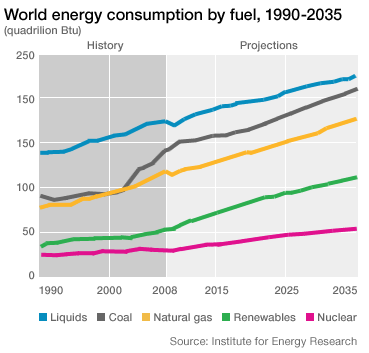
\includegraphics[width=0.33\textwidth]{test}
%        \caption{Caption}
%        \label{fig1}
%\end{figure}


\end{document}
